\documentclass[13pt, aspectratio=169]{beamer}
\usetheme{Copenhagen}
\usecolortheme{beaver}
\setbeamertemplate{navigation symbols}{}
\setbeamercovered{transparent}

\usepackage[utf8]{inputenc}
\usepackage{graphicx}
\usepackage{amsmath}
\usepackage{hyperref}
\usepackage{biblatex}
\usepackage{tikz}


\title{STUDI PENGARUH STACKING LAYER DAN VARIASI PARAMETER PADA
MODEL GRAFENA KANE-MELE}
\subtitle{Presentasi Proposal Skripsi}
\author{Akmal Suratmi}
\institute{Program Studi Fisika, Fakultas Matematika dan Ilmu Pengetahuan Alam, Universitas Hasanuddin}
\date{\today}
\begin{document}

\frame{\titlepage}
\begin{frame}
\frametitle{Outline}
\begin{itemize}
    \item Latar Belakang
    \item Tujuan Penelitian
    \item Model Penelitan 
    \item Metodologi Penelitian
\end{itemize}
\end{frame}

\section{Latar Belakang}
\begin{frame}
  \frametitle{Krisis Hukum Moore}
\begin{columns}
  \column{0.5\textwidth}
  \begin{coulumn}
    Limit miniaturisasi dan disipasi pada perangkat elektronik konvensional
    \begin{image}
      
\includegraphics[width=0.8\textwidth]{picture/disipation_data.jpg}
    \end{image}
  \end{coulumn}
  \pause
  \column{0.7\textwidth}
  \begin{image}
    
\includegraphics[width=0.8\textwidth]{picture/disipation_data.jpg.jpg}
  \end{image}
\end{columns} 
\end{frame}

% Solution from spintronics
\begin{frame}
\frametitle{Spintronics}
\begin{columns}
  \column{0.5\textwidth}
    \begin{image}
      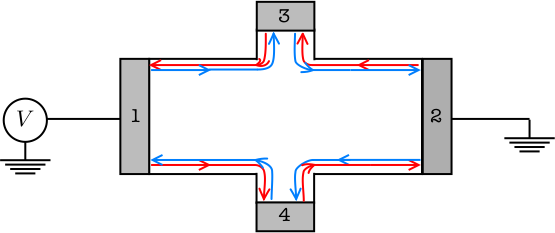
\includegraphics[width=0.8\textwidth]{picture/qsh_hallbar.png}
    \end{image}
    \pause
  \column{0.5\textwidth}
    \begin{image}
      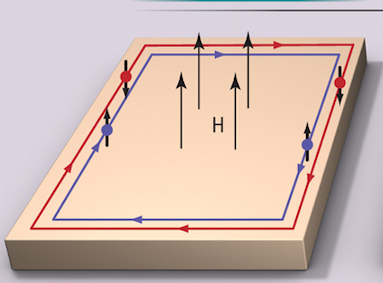
\includegraphics[width=0.8\textwidth]{picture/qhall-effect.png}
    \end{image}
\end{columns}
\end{frame}

\section{Tujuan Penelitian}
\begin{frame}
  \frametitle{Tujuan Penelitian}
  \begin{enumerate}
    \small
  \item  Memperoleh struktur pita ribbon pada model  \textit{stacking} grafena dengan \textit{hopping} antar lapisan yang menunjukkan perilaku efek tepi sistem.
  \item Memperoleh peta respon sistem  \textit{stacking} grafena terhadap perubahan parameter \textit{hopping} dan potensial kisi lewat analisis sturktur pita, kerapatan energi, dan probabilitas elektron.
  \item Memperoleh plot evolusi  \textit{ Hybrid Wannier Function Center} terhadap pergerakan ruang momentum searah dengan arah penumpukan lapisan.
  \item Memvalidasi keberadaan atau ketiadaan \textit{Surface State} pada permukaan grafena \textit{Stacking} dengan analisis perilaku magnetoelektrik atau \textit{Axion Angle}.
\end{enumerate}
\begin{itemize}

\end{itemize}
\end{frame}
\section{Metodologi Penelitian}
\begin{frame}
\frametitle{Struktur Kristal Grafena}
\begin{columns}[T, onlytextwidth]
  \begin{column}{0.5\textwidth}
    \centering
    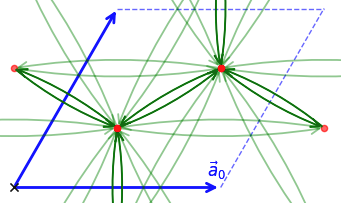
\includegraphics[width=\linewidth]{picture/graphene1.png}
  \end{column}
  \pause
  \begin{column}{0.5\textwidth}
    \centering
    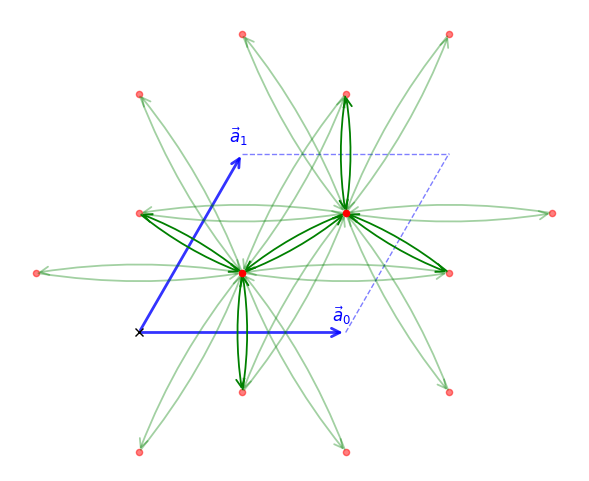
\includegraphics[width=\linewidth]{picture/graphene.png}
  \end{column}
\end{columns}
\end{frame}

\begin{frame}{Many-Body pada Sistem Kristal}
    \begin{columns}[T]
        \begin{column}{0.5\textwidth}
            \textbf{Hamiltonian Elektronik Eksplisit:}
            \begin{equation*}
                \hat{H}_e = \hat{T}_e + \hat{V}_{en} + \hat{V}_{ee}
            \end{equation*}
            \vspace{0.2cm}
            \pause
            Suku interaksi Coulomb antar elektron ($\hat{V}_{ee}$) menciptakan korelasi yang sangat kompleks:
            \begin{equation*}
                \hat{V}_{ee} = \frac{1}{2} \sum_i \sum_{j \neq i} \frac{1}{|\vec{r}_i - \vec{r}_j|}
            \end{equation*}
        \end{column}
       \pause 
        \begin{column}{0.5\textwidth}
            \begin{block}{The Curse of Dimensionality}
                \begin{itemize}
                    \item Kerapatan elektron pada grafena mencapai $\sim 10^{23}$ per cm$^2$.
                    \item Menghitung interaksi eksplisit setiap pasangan elektron membutuhkan sumber daya komputasi yang tumbuh secara eksponensial.
                    \item \textbf{Resolusi:} Diperlukan reduksi dari sistem $N$-partikel menjadi model partikel tunggal efektif.
                \end{itemize}
            \end{block}
        \end{column}
    \end{columns}
\end{frame}

\begin{frame}{Pendekatan Tight-Binding (LCAO) pada Grafena}
    \begin{columns}[T]
        \begin{column}{0.45\textwidth}
            \textbf{Lokalisasi Orbital $p_z$}
            \vspace{0.2cm}
            % Ganti 'graphene_orbitals.png' dengan file gambar/diagram TikZ kamu
            % \includegraphics[width=\linewidth]{graphene_orbitals.png}
            \begin{itemize}
                \item Ikatan $\sigma$ ($sp^2$) membentuk kerangka mekanik yang kaku.
                \item Sifat elektronik dekat level Fermi didominasi murni oleh elektron pada orbital $p_z$ (pita $\pi$).
            \end{itemize}
        \end{column}
       \pause 
        \begin{column}{0.55\textwidth}
            \begin{block}{Hamiltonian Tight-Binding Terreduksi}
                Mengabaikan interaksi jarak jauh, dinamika elektron disederhanakan menjadi parameter \textit{hopping} terdekat ($t \approx 2.8$ eV):
                \begin{equation*}
                    \hat{H}_{TB} = -t \sum_{\langle i,j \rangle, \sigma} \left( c_{i\sigma}^\dagger c_{j\sigma} + h.c. \right)
                \end{equation*}
                \vspace{0.1cm}
                \footnotesize{Di mana $c_{i\sigma}^\dagger$ menciptakan elektron dengan spin $\sigma$ di situs $i$. Model ini menjadi basis fundamental sebelum penambahan suku interaksi intrinsik seperti kopling Spin-Orbit.}
            \end{block}
        \end{column}
    \end{columns}
\end{frame}

\begin{frame}
  \frametitle{Kane-Mele Model}
  \begin{columns}[T]
    \begin{column}{0.45\textwidth}
      \begin{figure}
        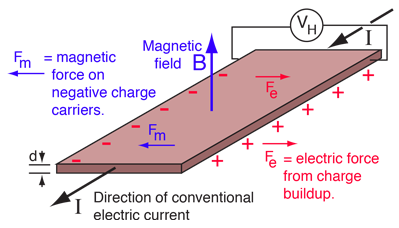
\includegraphics[width=1.0\textwidth]{picture/hall.png} 
      \end{figure}
    \end{column}
    \pause

    \begin{column}{0.55\textwidth}
      \begin{block}{Hamiltonian Kane-Mele}
        $$
  \mathcal{H}_{\text{KM},l} = t \sum_{\langle i,j \rangle,\sigma} c_{il\sigma}^\dagger c_{jl\sigma} 
+ i\lambda_{\text{SO}} \sum_{\langle\langle i,j \rangle\rangle,\sigma} \nu_{ij} c_{il\sigma}^\dagger s^z_{\sigma\sigma'} c_{jl\sigma'} \\
    + i\lambda_R \sum_{\langle i,j \rangle, \sigma \sigma'} c_{i\sigma}^\dagger (\mathbf{s} \times \hat{\mathbf{d}_{ij}})^z_{\sigma \sigma'}c_{j\sigma'}
+ \lambda_v \sum_{i,\sigma} \xi_i c_{il\sigma}^\dagger c_{il\sigma}
      $$
      \end{block}
    \end{column}
  \end{columns}
\end{frame}

\begin{frame}
  \begin{columns}[T]
    \begin{column}{0.45\textwidth}
      \begin{figure}
        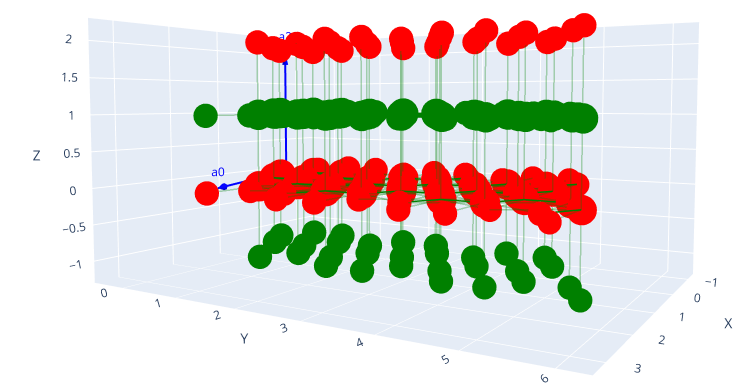
\includegraphics[width=1.0\textwidth]{picture/stacking_layer.png} 
      \end{figure}
    \end{column}

    \begin{column}{0.55\textwidth}
      \begin{block}
        $$ 
        \mathcal{H} = \underbrace{\sum_l \mathcal{H}_{\text{KM},l}}_{\text{Intralayer}} 
+ \underbrace{\tau \sum_{\langle l,l' \rangle} \sum_{i,\sigma} c_{il\sigma}^\dagger c_{il'\sigma}}_{\text{Hopping Antarlapisan}} \\
        + \underbrace{i\lambda_{SO\perp} \sum_{\langle l,l' \rangle} \sum_{i,\sigma,\sigma'} \mu_{ll'} c_{il\sigma}^\dagger s^z_{\sigma\sigma'} c_{il'\sigma'}}_{\text{Kopling Spin-Orbit Antarlapisan}},
        $$
      \end{block}
    \end{column}
  \end{columns}
\end{frame}

\begin{frame}
  \frametitle{Ekstraksi Nilai Fungsi Eigen}
  
  \begin{columns} % Hapus {0.45\textwidth} di sini
    
    \begin{column}{0.45\textwidth}
      \begin{block}{Schrodinger equation}
        \[
        \mathcal{H}\psi(r) = E\psi(r)
        \]
      \end{block}
     \pause 
      \begin{center}
        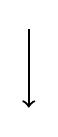
\begin{tikzpicture}
          \draw[->, thick] (0,1) -- (0,0);
        \end{tikzpicture}
      \end{center}
      Spektrum energi, Kerapatan energi, Probabilitas keberadaan elektron
    \end{column}
\pause
    \begin{column}{0.55\textwidth}
  \centering
  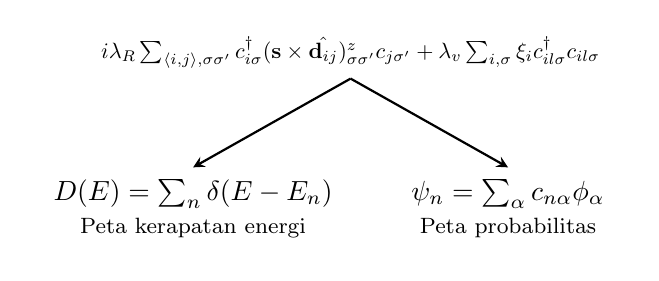
\begin{tikzpicture}[>=stealth, node distance=1.5cm]
    % Persamaan Utama (Atas/Pusat)
    \node (Hamiltonian) at (0,0) {
      \scalebox{0.8}{$i\lambda_R \sum_{\langle i,j \rangle, \sigma \sigma'} c_{i\sigma}^\dagger (\mathbf{s} \times \hat{\mathbf{d}_{ij}})^z_{\sigma \sigma'}c_{j\sigma'} + \lambda_v \sum_{i,\sigma} \xi_i c_{il\sigma}^\dagger c_{il\sigma}$}
    };
\pause
    % Node Kiri (Kerapatan Energi)
    \node (Density) at (-2, -2) {
      \begin{tabular}{c}
        $D(E) = \sum_{n} \delta(E - E_{n})$ \\
        \footnotesize Peta kerapatan energi
      \end{tabular}
    };
\pause
    % Node Kanan (Probabilitas)
    \node (Prob) at (2, -2) {
      \begin{tabular}{c}
        $\ket{\psi_{n}} = \sum_{\alpha} c_{n \alpha}\ket{\phi_{\alpha}}$ \\
        \footnotesize Peta probabilitas
      \end{tabular}
    };

    % Panah bercabang (Pohon Faktor)
    \draw[->, thick] (Hamiltonian.south) -- (Density.north);
    \draw[->, thick] (Hamiltonian.south) -- (Prob.north);
  \end{tikzpicture}
\end{column}
  \end{columns}
\end{frame}

\begin{frame}
  \frametitle{Analisis Hybrid Wannier Center}
  \begin{columns}[T]
    \begin{column}{0.45\textwidth}
    Bagaimana mendeteksi $Z_2$?
    \pause
    \begin{center}
      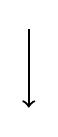
\begin{tikzpicture}
        \draw[->, thick] (0,1) -- (0,0);
      \end{tikzpicture}
    \end{center}
    
    Apakah ada perubahan ekspektasi posisi pusat muatan ketika terjadi perubahan dalam ruang momentum. 
    \pause
    \vspace{3em}
    
    \textcolor{blue}{\textbf{kenapa Hybrid Wannier Center?}}
    \end{column}
    \pause
    \begin{column}{0.55\textwidth}
      \begin{figure}
        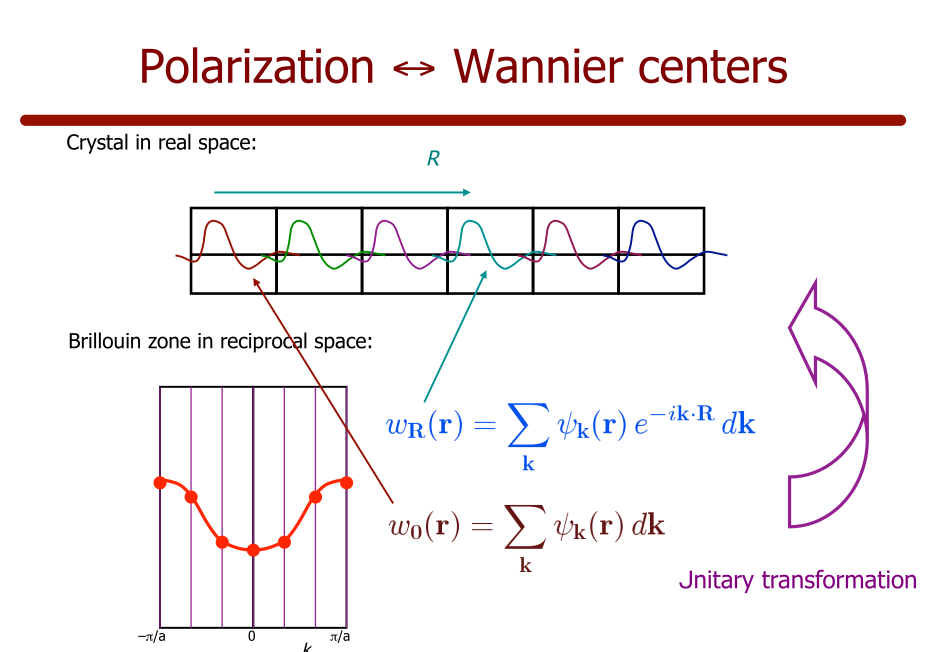
\includegraphics[width=1.0\textwidth]{picture/transformasi-blochWannier.png}
      \end{figure}
    \end{column}
  \end{columns}
\end{frame}

\begin{frame}
  \frametitle{Analisis Hybrid Wannier Center}
  \begin{columns}[T]
    \begin{column}{0.45\textwidth}
      ada masalah dengan \textit{gauge} pada Wannier centers
      \pause
      \[
        r|w_0 \rangle = \frac{V}{(2\pi)^3} \int_{BZ} dk ( - i \nabla_ke^{ik \cdot r} ) |\psi_k \rangle
      \]
    \end{column}
    \pause
    \begin{column}{0.55\textwidth}
      \[
r|w_0 \rangle = \frac{V}{(2\pi)^3} \int_{BZ} dk ( - i \nabla_ke^{i\beta(k)} ) |\psi_k \rangle \\
r|w_0 \rangle = \frac{V}{(2\pi)^3} \int_{BZ} dk \quad[( - i (i\nabla_k\beta(k))e^{i\beta(k)} ) |\psi_k \rangle \;   - i e^{i\beta(k)} \nabla_k|\psi_k \rangle] \\ 
      \]
    \end{column}
  \end{columns}
\end{frame}

\begin{frame}
  \frametitle{Analisis Axion Angel}
  \begin{columns}
    \begin{column}{0.5\textwidth}
      \textcolor{blue}{\textbf{Apakah penumpukan grafena memberikan efek Quantum spin hall yang berbeda dari satu lapisan?}}
      \pause 
      \begin{center}
      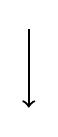
\begin{tikzpicture}
        \draw[->, thick] (0,1) -- (0,0);
      \end{tikzpicture}
      \end{center}
      Sama seperti efek hall dua dimensi yang memiliki efek tepi dimana ada arus pada tepian insulator, material hall tiga dimensi juga seharusnya memiliki efek arus pada tepian. \textbf{Cara untuk mendeteksi fenomena tersebut kita gunakan} \textcolor{blue}{\textbf{Axion Angel}}
    \end{column}
    \pause 
    \begin{column}{0.5\textwidth}
     \[
      \boxed{
\Delta \mathcal{L}_{EM} = \frac{\theta e^2}{2 \pi h}\mathbf{E. B} = \frac{\theta e^2}{16 \pi h} \epsilon^{\alpha \beta \gamma \delta}F_{\alpha \beta } F_{\gamma \delta}
}
     \]
     \vspace{2pt}
     \pause
     nilai theta hanya akan berarti ketika dia mengalami perubahan ketika mengalami pumping di ruang momentum.
    \end{column}
  \end{columns}
\end{frame}
\begin{frame}
  \frametitle{Analisis Axion Angel}
  
  \begin{columns}
    \begin{column}{0.45\textwidth}
    \[
        \theta = \frac{1}{2π} \int_{BZ} d^3k \quad\epsilon_{ijk} \mathbf{Tr}\left[ \mathcal{A}_{i}\partial_{j}\mathcal{A}_{k} - i \frac{2}{3} \mathcal{A}_{i} \mathcal{A}_{j}\mathcal{A}_{k} \right]
      \]
       \[ \bar{A}_n (\bar{k}) =  \langle n_k | \nabla_{\bar{R}} | n_k \rangle \]
      \pause 
      definisi ini membuat formulasi menjadi \textit{gauge dependent}
      \pause
      \[
        \mathcal{F}_{ij} = \partial_{i}\mathcal{A}_{j} - \partial_{j}\mathcal{A}_{i} - i[\mathcal{A_{i}A_{j}}]
      \]
      % arrow
      \begin{center}
      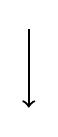
\begin{tikzpicture}
        \draw[->, thick] (0,1) -- (0,0);
      \end{tikzpicture} 
      \end{center}
      \begin{center}
        \textcolor{blue}{\textbf{Gauge invariant}}
      \end{center}
    \end{column}
    \begin{column}{0.55\textwidth} 
      \textcolor{blue}{\textbf{Bagaimana cara melihat perubahan theta?}}
      \pause
      \[
        \theta = \frac{1}{16 \pi}\int_{0}^{\beta}d\beta' \int d^3 k\; \epsilon_{ijkl} \mathbf{Tr}[\mathcal{F}_{ij}(\mathbf{k},\beta')\mathcal{F}_{kl}(\mathbf{k},\beta')]
      \]
    \end{column}
  \end{columns}
\end{frame}

\begin{frame}{Ekstensi Numerik}
    \begin{itemize}
        \item Implementasi model sistem memanfaatkan paket \textbf{PythTB 2.0} (Python) \parencite{Cole_Python_Tight_Binding_2025}.
        \item Dikembangkan khusus untuk mengonstruksi dan menganalisis model \textit{Tight-Binding} pada studi teoritikal material topologis.
        \item \textbf{Keunggulan:} Mereduksi kode numerik yang panjang menjadi baris singkat, sehingga menghemat waktu dan komputasi.
        \item \textbf{Empat fungsionalitas utama yang diadopsi:} 
        \begin{enumerate}
            \item Konstruksi model
            \item \textit{State sampling}
            \item Analisis topologi
            \item Visualisasi
        \end{enumerate}
    \end{itemize}
\end{frame}

\begin{frame}{Struktur dan Fungsionalitas Kode \texttt{PythTB}}
    \begin{table}
    \centering
    % Menyesuaikan ukuran tabel agar pas dengan lebar slide
    \resizebox{\textwidth}{!}{
    \begin{tabular}{@{}l l l@{}} 
    \toprule
    \textbf{Kode} & \textbf{Fungsi} & \textbf{Keluaran} \\ \midrule
    \texttt{Model-Hamiltonian.py} & Mengonstruksi model sistem \textit{tight-binding} & Fungsi objek model \\ \addlinespace
    \texttt{Peta-spektrum.py} & Memetakan pengaruh gangguan terhadap efek tepi & Visualisasi peta spektrum energi \\ \addlinespace
    \texttt{Peta-prob.py} & Memetakan pengaruh gangguan terhadap probabilitas elektron & Visualisasi distribusi probabilitas \\ \addlinespace
    \texttt{Dos.py} & Memetakan pengaruh gangguan terhadap \textit{Density of States} & Peta \textit{Density of States} (DOS) \\ \addlinespace
    \texttt{Hwf.py} & Menganalisis sifat topologi 3D via \textit{Wannier functions} & Plot evolusi \textit{Hybrid Wannier Centers} \\ \addlinespace
    \texttt{Axion-angle.py} & Menganalisis efek topologi melalui respon magnetoelektrik & Plot nilai $\theta$ terhadap parameter $\beta$ \\ \addlinespace
    \texttt{Visualisasi.py} & Melakukan pemetaan struktur geometri model & Representasi visual struktur kristal \\ \bottomrule
    \end{tabular}
    }
    \end{table}
\end{frame}

\begin{frame}{Diagram Alur Penelitian}
    \begin{figure}
    \centering
    % Menyesuaikan tinggi diagram agar tidak melebihi slide Beamer
    \resizebox{!}{0.85\textheight}{
    \begin{tikzpicture}[node distance=1.8cm, auto,
        % Definisi Style Blok
        startstop/.style={rectangle, rounded corners, minimum width=3cm, minimum height=1cm, text centered, draw=black, fill=red!10},
        process/.style={rectangle, minimum width=4cm, minimum height=1cm, text centered, draw=black, fill=blue!5},
        decision/.style={diamond, minimum width=3cm, minimum height=1cm, text centered, draw=black, fill=green!10, aspect=2},
        arrow/.style={thick,->,>=stealth},
        line/.style={thick,-}
    ]

    % Node - Node
    \node (start) [startstop] {Mulai};
    \node (lit) [process, below of=start] {Studi Literatur \& Parameterisasi ($t, \lambda_{SO}, \lambda_R$)};
    \node (model2d) [process, below of=lit] {Konstruksi Model 2D (Kane-Mele)};
    \node (stack) [process, below of=model2d] {Stacking Layer (3D Model)};
    \node (val) [decision, below of=stack, yshift=-0.5cm] {Validasi Efek Tepi?};
    \node (analisis) [process, below of=val, yshift=-0.5cm] {Analisis Respon Sistem};

    % Percabangan Analisis (Parallel)
    \node (spektrum) [process, below of=analisis, xshift=-3cm, text width=3.5cm] {Peta Spektrum \& Probabilitas\\(Deteksi \textit{Edge State})};
    \node (topologi) [process, below of=analisis, xshift=3cm, text width=3.5cm] {Analisis Topologi\\(HWC \& Axion $\theta$)};
    \node (kesimpulan) [process, below of=analisis, yshift=-3cm] {Interpretasi Fisik \& Kesimpulan};
    \node (stop) [startstop, below of=kesimpulan] {Selesai};

    % Garis Penghubung
    \draw [arrow] (start) -- (lit);
    \draw [arrow] (lit) -- (model2d);
    \draw [arrow] (model2d) -- (stack);
    \draw [arrow] (stack) -- (val);

    % Logika Decision
    \draw [arrow] (val) -- node[anchor=east] {Ya} (analisis);
    \draw [line] (val.east) -- ++(1.5,0) node[anchor=south] {Tidak};
    \draw [arrow] ($(val.east)+(1.5,0)$) |- (model2d.east);

    % Percabangan
    \draw [arrow] (analisis) -| (spektrum);
    \draw [arrow] (analisis) -| (topologi);

    % Penyatuan Kembali
    \draw [arrow] (spektrum) |- (kesimpulan);
    \draw [arrow] (topologi) |- (kesimpulan);
    \draw [arrow] (kesimpulan) -- (stop);

    \end{tikzpicture}
    }
    \end{figure}
\end{frame}

\begin{frame}{Skema Komputasi Numerik (PythTB)}
    \begin{figure}
    \centering
    % Menyesuaikan lebar diagram agar pas dengan slide
    \resizebox{!}{0.85\textheight}{
    \begin{tikzpicture}[node distance=1.5cm,
        % Definisi Style
        io/.style={trapezium, trapezium left angle=70, trapezium right angle=110, minimum width=3cm, minimum height=1cm, text centered, draw=black, fill=orange!10},
        process/.style={rectangle, minimum width=3cm, minimum height=1cm, text centered, draw=black, fill=cyan!5},
        subroutine/.style={rectangle, rounded corners, minimum width=3cm, minimum height=1cm, text centered, draw=black, dashed},
        arrow/.style={thick,->,>=stealth}
    ]

    % Input
    \node (param) [io] {Input Parameter ($H_{intralayer}, H_{interlayer}$)};

    % Core Process
    \node (pythtb) [process, below=0.8cm of param] {\textbf{PythTB Engine}\\(Konstruksi Hamiltonian)};

    % Output Intermediate
    \node (diag) [process, below=0.8cm of pythtb] {Diagonalisasi Matriks ($H\psi = E\psi$)};

    % Cabang Output
    \node (dos) [subroutine, below left=1.5cm and -1cm of diag, text width=3cm] {\texttt{Dos.py}\\Hitung Kerapatan Keadaan};
    \node (band) [subroutine, below=1.5cm of diag, text width=3cm] {\texttt{Peta-spektrum.py}\\Plot Pita Energi};
    \node (hwf) [subroutine, below right=1.5cm and -1cm of diag, text width=3cm] {\texttt{Hwf.py}\\Hitung Pusat Wannier (HWC)};

    % Final Result
    \node (visual) [io, below=4.5cm of diag, minimum width=8cm] {Visualisasi Data \& Grafik ($\theta$, $Z_2$, Bandgap)};

    % Garis
    \draw [arrow] (param) -- (pythtb);
    \draw [arrow] (pythtb) -- (diag);
    \draw [arrow] (diag) -| (dos);
    \draw [arrow] (diag) -- (band);
    \draw [arrow] (diag) -| (hwf);

    \draw [arrow] (dos) -- (visual.north -| dos);
    \draw [arrow] (band) -- (visual.north -| band);
    \draw [arrow] (hwf) -- (visual.north -| hwf);

    \end{tikzpicture}
    }
    \end{figure}
\end{frame}

\begin{frame}
  % sekian terima kasih
  \begin{center}
    \textcolor{blue}{\textbf{Sekian, Terima Kasih}}
  \end{center}
\end{frame}

\end{document}
